\section{Convolutional neural net}
\peng{
Given two functions $f,g:\{-n, \cdots, n\}\to \polR$, the discrete convolution is defined by
\[(f*g)(x) = \sum_{y = -n}^{n} f(y)g(x-y).\]
The ReLU net is defined by
\[ ReLU(t) = \max{0,t}.\]
The convolutional neural networks, denoted by ConvNets, consist of three different types of layers:
convolutional layer, pooling layer, and fully connected layer.
The architecture is of this form:
\[
\textrm{Input} \to 
\underbrace{[\textrm{Conv} \to \textrm{ReLU} \to \textrm{Pool]}}
_\textrm{N times} 
\to \textrm{FC}
\]
\textbf{PW: Need descriptions of the CONV, ReLU Pool and FC layers. 
Resource: \url{http://cs231n.github.io/convolutional-networks/}}

After applying the fully-connected layer, we obtain a vector of scores 
$\mathbf v(x) = (v_1(x), \cdots v_n(x))$. 
We first apply the soft-max
\[ (\mu_1(x),\cdots, \mu_n(x)) 
= SM(x) = \left( \frac{e^{v_1}}{\sum_i e^{v_i}}, 
\cdots  \frac{e^{v_n}}{\sum_i e^{v_i}}  \right). \]
The cross entropy loss function is defined as
\[\mathcal L (x) = -\sum_{j = 1}^n \log(\frac{e^{v_j}}{\sum_i e^{v_i}}).  \]

}
\begin{figure}[t!]
	\centering
	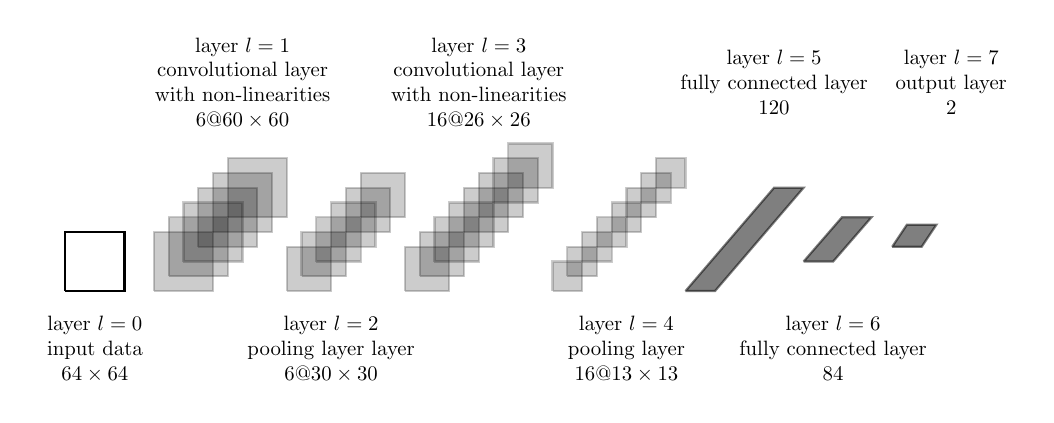
\begin{tikzpicture}[thick,scale=0.75, every node/.style={scale=0.75}]
		\node at (0.5,-1){\begin{tabular}{c}layer $l = 0$\\input data\\ $64\times 64$ \end{tabular}};
		
		\draw (0,0) -- (1,0) -- (1,1) -- (0,1) -- (0,0);
		
		\node at (3,3.5){\begin{tabular}{c}layer $l = 1$\\convolutional layer\\with non-linearities\\$6@60\times 60$\end{tabular}};
		
		\draw[fill=black,opacity=0.2,draw=black] (2.75,1.25) -- (3.75,1.25) -- (3.75,2.25) -- (2.75,2.25) -- (2.75,1.25);
		\draw[fill=black,opacity=0.2,draw=black] (2.5,1) -- (3.5,1) -- (3.5,2) -- (2.5,2) -- (2.5,1);
		\draw[fill=black,opacity=0.2,draw=black] (2.25,0.75) -- (3.25,0.75) -- (3.25,1.75) -- (2.25,1.75) -- (2.25,0.75);
		\draw[fill=black,opacity=0.2,draw=black] (2,0.5) -- (3,0.5) -- (3,1.5) -- (2,1.5) -- (2,0.5);
		\draw[fill=black,opacity=0.2,draw=black] (1.75,0.25) -- (2.75,0.25) -- (2.75,1.25) -- (1.75,1.25) -- (1.75,0.25);
		\draw[fill=black,opacity=0.2,draw=black] (1.5,0) -- (2.5,0) -- (2.5,1) -- (1.5,1) -- (1.5,0);
		
		\node at (4.5,-1){\begin{tabular}{c}layer $l = 2$\\pooling layer layer\\$6@30\times30$\end{tabular}};
		
		\draw[fill=black,opacity=0.2,draw=black] (5,1.25) -- (5.75,1.25) -- (5.75,2) -- (5,2) -- (5,1.25);
		\draw[fill=black,opacity=0.2,draw=black] (4.75,1) -- (5.5,1) -- (5.5,1.75) -- (4.75,1.75) -- (4.75,1);
		\draw[fill=black,opacity=0.2,draw=black] (4.5,0.75) -- (5.25,0.75) -- (5.25,1.5) -- (4.5,1.5) -- (4.5,0.75);
		\draw[fill=black,opacity=0.2,draw=black] (4.25,0.5) -- (5,0.5) -- (5,1.25) -- (4.25,1.25) -- (4.25,0.5);
		\draw[fill=black,opacity=0.2,draw=black] (4,0.25) -- (4.75,0.25) -- (4.75,1) -- (4,1) -- (4,0.25);
		\draw[fill=black,opacity=0.2,draw=black] (3.75,0) -- (4.5,0) -- (4.5,0.75) -- (3.75,0.75) -- (3.75,0);
		
		\node at (7,3.5){\begin{tabular}{c}layer $l = 3$\\convolutional layer\\with non-linearities\\$16@26\times26$\end{tabular}};
		
		\draw[fill=black,opacity=0.2,draw=black] (7.5,1.75) -- (8.25,1.75) -- (8.25,2.5) -- (7.5,2.5) -- (7.5,1.75);
		\draw[fill=black,opacity=0.2,draw=black] (7.25,1.5) -- (8,1.5) -- (8,2.25) -- (7.25,2.25) -- (7.25,1.5);
		\draw[fill=black,opacity=0.2,draw=black] (7,1.25) -- (7.75,1.25) -- (7.75,2) -- (7,2) -- (7,1.25);
		\draw[fill=black,opacity=0.2,draw=black] (6.75,1) -- (7.5,1) -- (7.5,1.75) -- (6.75,1.75) -- (6.75,1);
		\draw[fill=black,opacity=0.2,draw=black] (6.5,0.75) -- (7.25,0.75) -- (7.25,1.5) -- (6.5,1.5) -- (6.5,0.75);
		\draw[fill=black,opacity=0.2,draw=black] (6.25,0.5) -- (7,0.5) -- (7,1.25) -- (6.25,1.25) -- (6.25,0.5);
		\draw[fill=black,opacity=0.2,draw=black] (6,0.25) -- (6.75,0.25) -- (6.75,1) -- (6,1) -- (6,0.25);
		\draw[fill=black,opacity=0.2,draw=black] (5.75,0) -- (6.5,0) -- (6.5,0.75) -- (5.75,0.75) -- (5.75,0);
		
		\node at (9.5,-1){\begin{tabular}{c}layer $l = 4$\\pooling layer\\$16@13\times13$\end{tabular}};
		
		\draw[fill=black,opacity=0.2,draw=black] (10,1.75) -- (10.5,1.75) -- (10.5,2.25) -- (10,2.25) -- (10,1.75);
		\draw[fill=black,opacity=0.2,draw=black] (9.75,1.5) -- (10.25,1.5) -- (10.25,2) -- (9.75,2) -- (9.75,1.5);
		\draw[fill=black,opacity=0.2,draw=black] (9.5,1.25) -- (10,1.25) -- (10,1.75) -- (9.5,1.75) -- (9.5,1.25);
		\draw[fill=black,opacity=0.2,draw=black] (9.25,1) -- (9.75,1) -- (9.75,1.5) -- (9.25,1.5) -- (9.25,1);
		\draw[fill=black,opacity=0.2,draw=black] (9,0.75) -- (9.5,0.75) -- (9.5,1.25) -- (9,1.25) -- (9,0.75);
		\draw[fill=black,opacity=0.2,draw=black] (8.75,0.5) -- (9.25,0.5) -- (9.25,1) -- (8.75,1) -- (8.75,0.5);
		\draw[fill=black,opacity=0.2,draw=black] (8.5,0.25) -- (9,0.25) -- (9,0.75) -- (8.5,0.75) -- (8.5,0.25);
		\draw[fill=black,opacity=0.2,draw=black] (8.25,0) -- (8.75,0) -- (8.75,0.5) -- (8.25,0.5) -- (8.25,0);
		
		\node at (12,3.5){\begin{tabular}{c}layer $l = 5$\\fully connected layer\\ $120$\end{tabular}};
		
		\draw[fill=black,draw=black,opacity=0.5] (10.5,0) -- (11,0) -- (12.5,1.75) -- (12,1.75) -- (10.5,0);
		
		\node at (13,-1){\begin{tabular}{c}layer $l = 6$\\fully connected layer\\$84$\end{tabular}};
		
		\draw[fill=black,draw=black,opacity=0.5] (12.5,0.5) -- (13,0.5) -- (13.65,1.25) -- (13.15,1.25) -- (12.5,0.5);
		
		\node at (15,3.5){\begin{tabular}{c} layer $l = 7$\\output layer\\$2$\end{tabular}};
		
		\draw[fill=black,draw=black,opacity=0.5] (14,0.75) -- (14.5,0.75) -- (14.75,1.125) -- (14.25,1.125) -- (14,0.75);
		
	\end{tikzpicture}
	\caption[Architecture of our convolutional neural network.]
	{The architecture of our convolutional neural network. 
	The convolutional layers (layers 1 and 3) actually represent two layers, with the ReLU net hidden, thus they already include non-linearities. 
	The output layer uses softmax activation functions.}
	\label{fig:traditional-convolutional-network}
\end{figure}


